\documentclass[a4paper,12pt]{article}
\usepackage{amssymb}
\usepackage{amsmath}
\usepackage[utf8]{inputenc}
\usepackage[german]{babel}
\usepackage[T1]{fontenc}
\usepackage[margin=2.5cm]{geometry}
\usepackage{booktabs}
\usepackage{hyperref}
\usepackage{eurosym}
\usepackage{rotating}
\usepackage{fancyhdr}
\usepackage{pdflscape}



\usepackage{color}
\definecolor{codegreen}{rgb}{0,0.6,0}
\definecolor{codegray}{rgb}{0.5,0.5,0.5}
\definecolor{codepurple}{rgb}{0.58,0,0.82}
\definecolor{backcolour}{rgb}{0.95,0.95,0.92}

\usepackage{listings}
\lstdefinestyle{C}{
	backgroundcolor=\color{backcolour},   
	commentstyle=\color{codegreen},
	keywordstyle=\color{magenta},
	numberstyle=\tiny\color{codegray},
	stringstyle=\color{codepurple},
	basicstyle=\footnotesize,
	breakatwhitespace=false,         
	breaklines=true,                 
	captionpos=b,                    
	keepspaces=true,                 
	numbers=left,                    
	numbersep=5pt,                  
	showspaces=false,                
	showstringspaces=false,
	showtabs=false,
	frame=single,                  
	tabsize=4
}

\newcommand{\VID}{0x1209}
\newcommand{\PID}{0x2222}

\title{Signalgenerator}
\author{Hendrik Lüth}

\begin{document}

\begin{center}
\textsc{\LARGE Elektroniker für Geräte und Systeme \\[0.5cm] Betrieblicher Auftrag 2015}\\[1cm]

\newcommand{\HRule}{\rule{\linewidth}{0.5mm}}
\HRule \\[0.4cm]
{ \huge \bfseries DDS-Signalgenerator}\\[0.4cm]

\HRule \\[1cm]


\includegraphics[width=0.35\textwidth]{./img/Wappen_MSM.jpg}\\[1cm]    

\textsc{\LARGE Hendrik Lüth \\ Prüflingsnummer: 20050}\\[0.5cm]

\textsc{\Large Schleswiger Str. 21 \\ 24392 Süderbrarup}\\[1.5cm]

\hfill


\begin{minipage}{0.5\textwidth}
\begin{flushleft} \large
\emph{Ausbildungsbetrieb:}\\
Ausbildungswerkstatt der Marine\\
Mürwiker Str. 203\\
24944 Flensburg\\
Tel.Nr: 046131355080
\end{flushleft}
\end{minipage}
\hfill
\begin{minipage}{0.4\textwidth}
\begin{flushright} \large
\hfill
\emph{Projektbetreuer:} \\
Bastian Kaul\\
Tel.Nr: 046131355081
\end{flushright}
\end{minipage}

\end{center}
\pagebreak
~ \\

\pagebreak
\tableofcontents
\pagebreak
\pagestyle{fancy}
\lhead{Hendrik Lüth}
\chead{Signalgenerator}
\rhead{\today}
\lfoot{ABW Flensburg}
\cfoot{\thepage}
\rfoot{Betrieblicher Auftrag}
\renewcommand{\headrulewidth}{0.4pt} 
\renewcommand{\footrulewidth}{0.4pt} 

\begin{center}
\section*{Arbeitsablaufplan Signalgenerator}
Projektleiter: Hendrik Lüth \qquad Projektzeitraum: 01.05.2015 - 31.05.2015
\medskip

\begin{tabular}{lp{15cm}|r|r|}
\hline
\multicolumn{1}{|c|}{Pos.} & Arbeitsschritt & ~~Soll~~ & ~~Ist~~ \\ \hline
\multicolumn{1}{|c|}{1} & Anfertigung eines Arbeitsablaufplans & 1,0h &  \\ \hline
\multicolumn{1}{|c|}{2} & Schreiben eines Lastenheftes für die Herstellung des Signalgenerators & 2,5h &  \\ \hline
\multicolumn{1}{|c|}{3} & Anfertigung eines Inbetriebnahmeprotokolls für den Signalgenerator & 2,5h &  \\ \hline
\multicolumn{1}{|c|}{4} & Schreiben eines Lastenheftes für die Herstellung des Gehäuses & 2,0h &  \\ \hline
\multicolumn{1}{|c|}{5} & Anfertigung eines Abnahmeprotokolls für das Gehäuse & 0,5h &  \\ \hline
\multicolumn{1}{|c|}{6} & Ausfüllen des Inbetriebnahmeprotokolls für den Signalgenerator & 1,0h &  \\ \hline
\multicolumn{1}{|c|}{7} & Ausfüllen des Abnahmeprotokolls des Gehäuses & 1,0h &  \\ \hline
\multicolumn{1}{|c|}{8} & Montage des Signalgenerators in das Gehäuse & 0.5h &  \\ \hline
\multicolumn{1}{|c|}{9} & Aufstellen einer Kostenübersicht des Projektes & 3,0h &  \\ \hline
                       &  & 13,0h &  \\ \cline{3-4} 
\end{tabular}
 
\end{center}

\documentclass[a4paper,12pt]{article}
\usepackage{amssymb} % needed for math
\usepackage{amsmath} % needed for math
\usepackage[utf8]{inputenc} % this is needed for german umlauts
\usepackage[ngerman]{babel} % this is needed for german umlauts
\usepackage[T1]{fontenc}    % this is needed for correct output of umlauts in pdf
\usepackage[margin=2.5cm]{geometry} %layout
\usepackage{booktabs}

% this is needed for forms and links within the text
\usepackage{hyperref}  

% glossar, see http://en.wikibooks.org/wiki/LaTeX/Glossary
% has to be loaded AFTER hyperref so that entries are clickable
\usepackage[nonumberlist]{glossaries} 

% The following is needed in order to make the code compatible
% with both latex/dvips and pdflatex.
\ifx\pdftexversion\undefined
\usepackage[dvips]{graphicx}
\else
\usepackage[pdftex]{graphicx}
\DeclareGraphicsRule{*}{mps}{*}{}
\fi

\makeglossary 

%%%%%%%%%%%%%%%%%%%%%%%%%%%%%%%%%%%%%%%%%%%%%%%%%%%%%%%%%%%%%%%%%%%%%%
% Variablen                                 						 %
%%%%%%%%%%%%%%%%%%%%%%%%%%%%%%%%%%%%%%%%%%%%%%%%%%%%%%%%%%%%%%%%%%%%%%
\newcommand{\authorName}{Hendrik Lüth}
\newcommand{\Arbeitgeber}{Ausbildungswerkstatt der Marine}
\newcommand{\projekt}{DDS-Signalgenerator}


%%%%%%%%%%%%%%%%%%%%%%%%%%%%%%%%%%%%%%%%%%%%%%%%%%%%%%%%%%%%%%%%%%%%%%
% PDF Meta information                                 				 %
%%%%%%%%%%%%%%%%%%%%%%%%%%%%%%%%%%%%%%%%%%%%%%%%%%%%%%%%%%%%%%%%%%%%%%
\hypersetup{
  pdfauthor   = {\authorName},
  pdfkeywords = {\tags},
  pdftitle    = {\projektName~(Lastenheft)}
} 
 
%%%%%%%%%%%%%%%%%%%%%%%%%%%%%%%%%%%%%%%%%%%%%%%%%%%%%%%%%%%%%%%%%%%%%%
% Create a shorter version for tables. DO NOT CHANGE               	 %
%%%%%%%%%%%%%%%%%%%%%%%%%%%%%%%%%%%%%%%%%%%%%%%%%%%%%%%%%%%%%%%%%%%%%%
\newcommand\addrow[2]{#1 &#2\\ }

\newcommand\addheading[2]{#1 &#2\\ \hline}
\newcommand\tabularhead{\begin{tabular}{lp{13cm}}
\hline
}

\newcommand\addmulrow[2]{ \begin{minipage}[t][][t]{2.5cm}#1\end{minipage}% 
   &\begin{minipage}[t][][t]{8cm}
    \begin{enumerate} #2   \end{enumerate}
    \end{minipage}\\ }

\newenvironment{usecase}{\tabularhead}
{\hline\end{tabular}}




%%%%%%%%%%%%%%%%%%%%%%%%%%%%%%%%%%%%%%%%%%%%%%%%%%%%%%%%%%%%%%%%%%%%%%
% THE DOCUMENT BEGINS             	                              	 %
%%%%%%%%%%%%%%%%%%%%%%%%%%%%%%%%%%%%%%%%%%%%%%%%%%%%%%%%%%%%%%%%%%%%%%
\begin{document}
 \pagenumbering{roman}
 \input{Deckblatt}         % Deckblatt.tex laden und einfügen
 \setcounter{page}{2}
 \tableofcontents          % Inhaltsverzeichnis ausgeben
 \clearpage
 \pagenumbering{arabic}
 
\section{Zielbestimmung}
%%%%%%%%%%%%%%%%%%%%%%%%%%%%%%%%%%%%%%%%%%%%%%%%%%%%%%%%%%%%%%%%%%%%%%
% Warum wird das Projekt gemacht?           						 %
%%%%%%%%%%%%%%%%%%%%%%%%%%%%%%%%%%%%%%%%%%%%%%%%%%%%%%%%%%%%%%%%%%%%%%


\section{Produkteinsatz}
%%%%%%%%%%%%%%%%%%%%%%%%%%%%%%%%%%%%%%%%%%%%%%%%%%%%%%%%%%%%%%%%%%%%%%
% Wer ist die Zielgruppe?                   						 %
%%%%%%%%%%%%%%%%%%%%%%%%%%%%%%%%%%%%%%%%%%%%%%%%%%%%%%%%%%%%%%%%%%%%%%


\section{Funktionale Anforderungen}
%%%%%%%%%%%%%%%%%%%%%%%%%%%%%%%%%%%%%%%%%%%%%%%%%%%%%%%%%%%%%%%%%%%%%%
% Was muss das Programm können?                   					 %
%%%%%%%%%%%%%%%%%%%%%%%%%%%%%%%%%%%%%%%%%%%%%%%%%%%%%%%%%%%%%%%%%%%%%%
\begin{usecase}
  \addheading{Nummer}{Beschreibung} 
  \addrow{}{}
  \addrow{}{}
  \addrow{}{}
\end{usecase}

\section{Produktdaten}
%%%%%%%%%%%%%%%%%%%%%%%%%%%%%%%%%%%%%%%%%%%%%%%%%%%%%%%%%%%%%%%%%%%%%%
% Auf welchen Daten arbeitet das Produkt?                            %
%%%%%%%%%%%%%%%%%%%%%%%%%%%%%%%%%%%%%%%%%%%%%%%%%%%%%%%%%%%%%%%%%%%%%%
\begin{usecase}
  \addheading{Nummer}{Beschreibung} 
  \addrow{}{}
  \addrow{}{}
  \addrow{}{}
\end{usecase}

\section{Systemmodelle}
\subsection{Szenarien}
\subsection{Anwendungsfälle}

\clearpage
\input{Glossar} 
\end{document}

\section[Pflichtenheft betriebl. Auftrag]{Pflichtenheft des betrieblichen Auftrages}
Es soll ein Signalgenerator nach dem vorgegebenen Schaltplan hergestellt werden. Die PC-Software wird vom Auftraggeber bereitgestellt. Die Aufträge für die Herstellung des Gehäuses und des Signalgenerators werden an externe Auftragsnehmer vergeben. Als Gehäuse soll das Gehäuse \glqq GEH KS 21\grqq von Reichelt Elektronik genutzt werden. Die Kommunikation zwischen Computer und Signalgenerator ist im Kommunikationsprotokoll im Anhang spezifiziert. Dieses wird an den Auftragsnehmer zur Herstellung des Signalgenerators zum programmieren einer Firmware weitergegeben.\\
\bigskip
Der Auftragsnehmer wird folgende Tätigkeiten ausführen:
\begin{itemize}
\item Auswahl der Auftragsnehmer und schreiben der Lastenhefte der Teilaufträge
\item Anfertigung eines Datenblattes
\item Erstellen einer Kostenübersicht
\item Erstellen eines Inbetriebnahme-Protokolls
\item Erstellen eines Arbeitsablaufplanes
\item Funktionsprüfung des Signalgenerators
\item Erstellung einer Zeichnung zur Darstellung der Gehäuseänderungen
\item Erstellen eines Übergabeprotokolls
\item Einbau des Signalgenerators in das Gehäuse
\end{itemize}
\bigskip
Mit der Herstellung des Signalgenerators wird Werkstatt 2 beauftragt. Folgende Anforderungen müssen erfüllt werden:\\
\begin{itemize}
\item Zeichnen eines Layoutes auf Grundlage des Schaltplanes
\item Herstellen einer Platine, welche in das oben genannte Gehäuse passt
\item Beschaffen der verwendeten Bauteile
\item Bestücken der Platine
\item Testen der Platine anhand der Messvorgaben
\item Programmieren der Firmware des Mikrocontrollers
\end{itemize}
\bigskip
Mit der Herstellung des Gehäuses wird Werkstatt 1 beauftragt. Folgende Anforderungen werden gestellt werden:\\
\begin{itemize}
\item Beschaffen des Gehäuses
\item Herstellung des Gehäuses nach den vorgegebenen Zeichnungen.
\end{itemize}
\bigskip
Für den Auftrag wird ein Stundenkontingent von 20 Stunden veranschlagt. Sollte der Schaltplan fehlerhaft sein, so sind diese Fehler, nach Möglichkeit, zu korrigieren. Sollten Fehler in der mitgelieferten Software sein, so sind diese im Übergabeprotokoll zu vermerken.\\
\bigskip \\
\bigskip \\
\rule{5cm}{0.5mm}\\
Datum/Unterschrift Hendrik Lüth\\
\bigskip \\
\bigskip \\
\rule{5cm}{0.5mm}\\
Datum/Unterschrift Auftraggeber



\section[Datenblatt Signalgenerator]{Datenblatt des DDS-Signalgenerators}



\begin{minipage}{0.4\textwidth}
\begin{flushleft}
\subsection{Features}
Der Signalgenerator basiert auf dem Prinzip der Direkten Digitalen Synthese (DDS) und ist in der Lage, Ausgangs ein breites Spektrum an Frequenzen, Signalformen und Ausgangsspannungen zu erzeugen. Die Steuerung des Gerätes erfolgt ausschließlich über den Computer, ein autarker Betrieb ist möglich. Im Gerät können hardwarespezifische Kalibrierungswerte gespeichert werden.
\end{flushleft}
\end{minipage}
\hfill
\begin{minipage}{0.58\textwidth}
\begin{flushright}
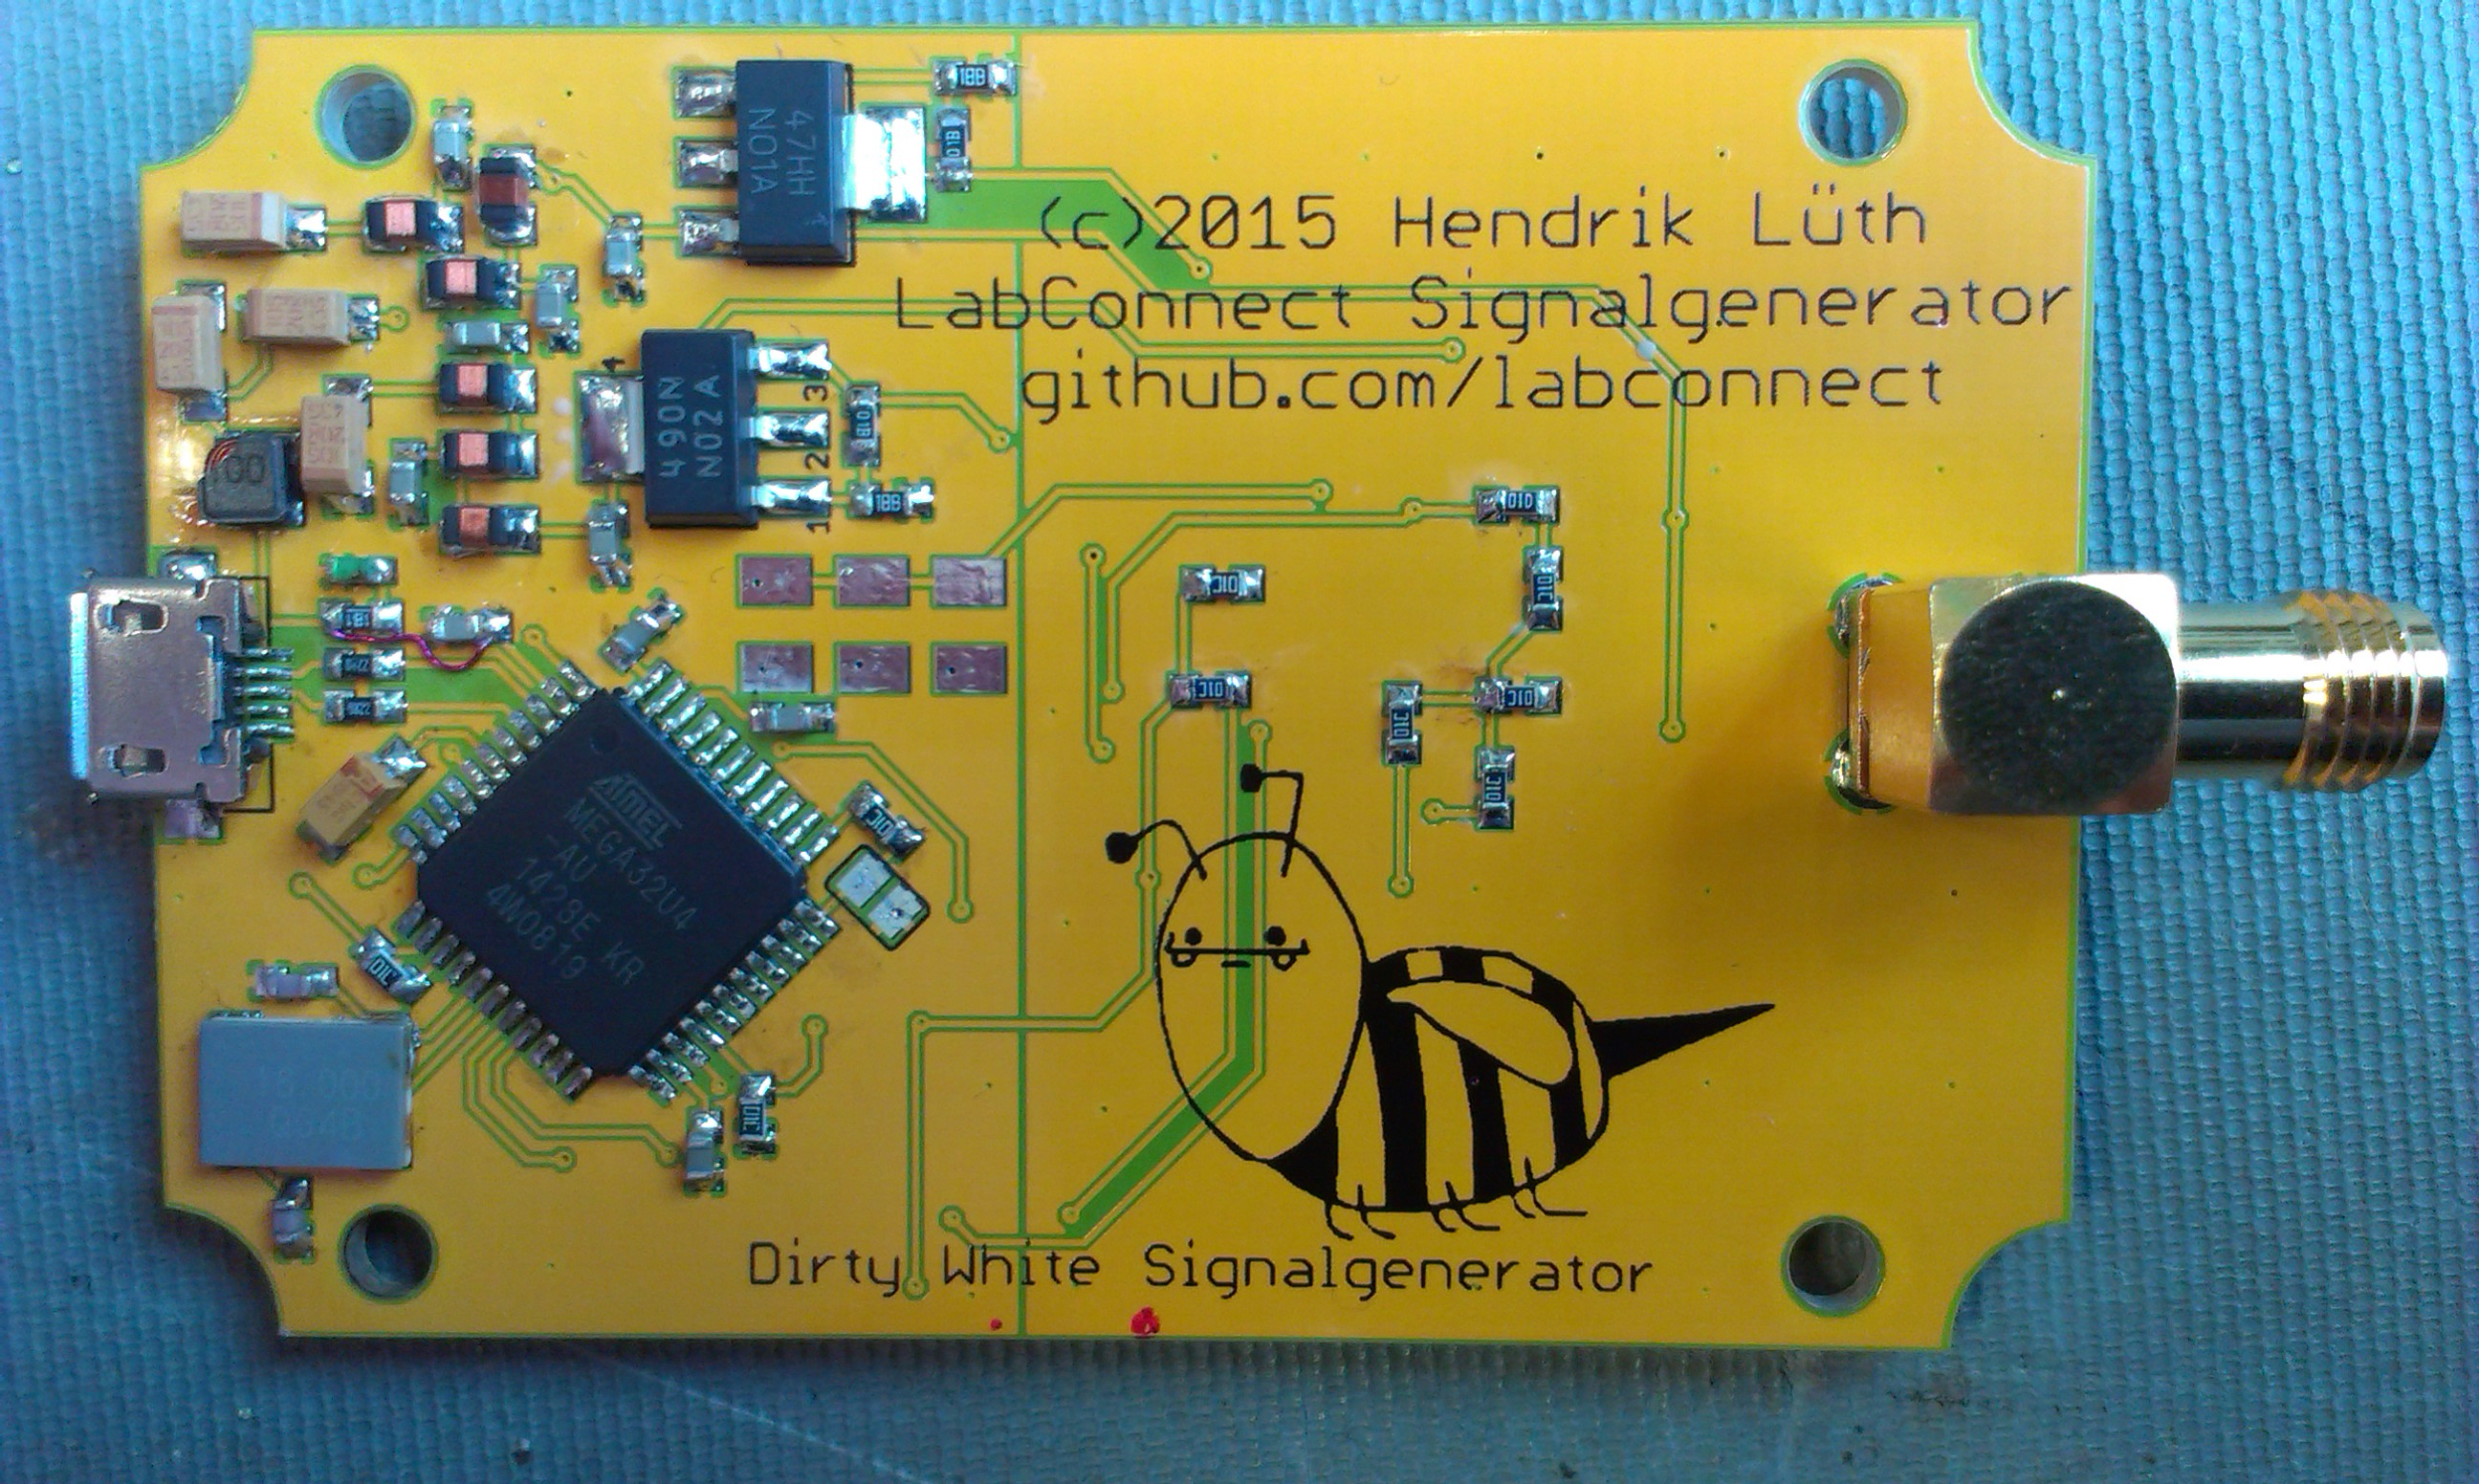
\includegraphics[width=\textwidth]{./img/FotoSgen.jpg}
\end{flushright}
\end{minipage}
\subsection{Eigenschaften}
\begin{center}
\begin{tabular}{l|ccc|c|l}
\hline
\textbf{Parameter} & \textbf{~~Min~~} & \textbf{~~Typ~~} & \textbf{~~Max~~} & \textbf{Einheit} & \textbf{Testbedingungen} \\
\hline
Betriebsspannung $U_{B}$ & 4,7 & 5 & 5,5 & Volt & \\
Stromaufnahme $I_{ges.}$ & 30 & 50 & 100 & mA & $U_{B}$=5V \\
Leistungsaufnahme P & 0,14 & 0,25 & 0,55 & W & \\
\hline
\end{tabular}
\end{center}

\subsection{Absolute Maximum Ratings}
\begin{center}
\begin{tabular}{l|c|c}
\hline
\textbf{Parameter} & \textbf{~~Max~~} & \textbf{Einheit} \\
\hline
Betriebsspannung $U_{B}$ & 6 & Volt \\
Spannung an D+ $U_{D+}$ & 3,6 & Volt \\
Spannung an D- $U_{D-}$ & 3,6 & Volt \\
\hline
Ausgangsstrom $I_{a}$ & 95 & mA \\
\end{tabular}
\end{center}


\documentclass[a4paper,12pt]{article}
\usepackage{amssymb} % needed for math
\usepackage{amsmath} % needed for math
\usepackage[utf8]{inputenc} % this is needed for german umlauts
\usepackage[ngerman]{babel} % this is needed for german umlauts
\usepackage[T1]{fontenc}    % this is needed for correct output of umlauts in pdf
\usepackage[margin=2.5cm]{geometry} %layout
\usepackage{booktabs}

% this is needed for forms and links within the text
\usepackage{hyperref}  

% glossar, see http://en.wikibooks.org/wiki/LaTeX/Glossary
% has to be loaded AFTER hyperref so that entries are clickable
\usepackage[nonumberlist]{glossaries} 

% The following is needed in order to make the code compatible
% with both latex/dvips and pdflatex.
\ifx\pdftexversion\undefined
\usepackage[dvips]{graphicx}
\else
\usepackage[pdftex]{graphicx}
\DeclareGraphicsRule{*}{mps}{*}{}
\fi

\makeglossary 

%%%%%%%%%%%%%%%%%%%%%%%%%%%%%%%%%%%%%%%%%%%%%%%%%%%%%%%%%%%%%%%%%%%%%%
% Variablen                                 						 %
%%%%%%%%%%%%%%%%%%%%%%%%%%%%%%%%%%%%%%%%%%%%%%%%%%%%%%%%%%%%%%%%%%%%%%
\newcommand{\authorName}{Hendrik Lüth}
\newcommand{\Arbeitgeber}{Ausbildungswerkstatt der Marine}
\newcommand{\projekt}{DDS-Signalgenerator}


%%%%%%%%%%%%%%%%%%%%%%%%%%%%%%%%%%%%%%%%%%%%%%%%%%%%%%%%%%%%%%%%%%%%%%
% PDF Meta information                                 				 %
%%%%%%%%%%%%%%%%%%%%%%%%%%%%%%%%%%%%%%%%%%%%%%%%%%%%%%%%%%%%%%%%%%%%%%
\hypersetup{
  pdfauthor   = {\authorName},
  pdfkeywords = {\tags},
  pdftitle    = {\projektName~(Lastenheft)}
} 
 
%%%%%%%%%%%%%%%%%%%%%%%%%%%%%%%%%%%%%%%%%%%%%%%%%%%%%%%%%%%%%%%%%%%%%%
% Create a shorter version for tables. DO NOT CHANGE               	 %
%%%%%%%%%%%%%%%%%%%%%%%%%%%%%%%%%%%%%%%%%%%%%%%%%%%%%%%%%%%%%%%%%%%%%%
\newcommand\addrow[2]{#1 &#2\\ }

\newcommand\addheading[2]{#1 &#2\\ \hline}
\newcommand\tabularhead{\begin{tabular}{lp{13cm}}
\hline
}

\newcommand\addmulrow[2]{ \begin{minipage}[t][][t]{2.5cm}#1\end{minipage}% 
   &\begin{minipage}[t][][t]{8cm}
    \begin{enumerate} #2   \end{enumerate}
    \end{minipage}\\ }

\newenvironment{usecase}{\tabularhead}
{\hline\end{tabular}}




%%%%%%%%%%%%%%%%%%%%%%%%%%%%%%%%%%%%%%%%%%%%%%%%%%%%%%%%%%%%%%%%%%%%%%
% THE DOCUMENT BEGINS             	                              	 %
%%%%%%%%%%%%%%%%%%%%%%%%%%%%%%%%%%%%%%%%%%%%%%%%%%%%%%%%%%%%%%%%%%%%%%
\begin{document}
 \pagenumbering{roman}
 \input{Deckblatt}         % Deckblatt.tex laden und einfügen
 \setcounter{page}{2}
 \tableofcontents          % Inhaltsverzeichnis ausgeben
 \clearpage
 \pagenumbering{arabic}
 
\section{Zielbestimmung}
%%%%%%%%%%%%%%%%%%%%%%%%%%%%%%%%%%%%%%%%%%%%%%%%%%%%%%%%%%%%%%%%%%%%%%
% Warum wird das Projekt gemacht?           						 %
%%%%%%%%%%%%%%%%%%%%%%%%%%%%%%%%%%%%%%%%%%%%%%%%%%%%%%%%%%%%%%%%%%%%%%


\section{Produkteinsatz}
%%%%%%%%%%%%%%%%%%%%%%%%%%%%%%%%%%%%%%%%%%%%%%%%%%%%%%%%%%%%%%%%%%%%%%
% Wer ist die Zielgruppe?                   						 %
%%%%%%%%%%%%%%%%%%%%%%%%%%%%%%%%%%%%%%%%%%%%%%%%%%%%%%%%%%%%%%%%%%%%%%


\section{Funktionale Anforderungen}
%%%%%%%%%%%%%%%%%%%%%%%%%%%%%%%%%%%%%%%%%%%%%%%%%%%%%%%%%%%%%%%%%%%%%%
% Was muss das Programm können?                   					 %
%%%%%%%%%%%%%%%%%%%%%%%%%%%%%%%%%%%%%%%%%%%%%%%%%%%%%%%%%%%%%%%%%%%%%%
\begin{usecase}
  \addheading{Nummer}{Beschreibung} 
  \addrow{}{}
  \addrow{}{}
  \addrow{}{}
\end{usecase}

\section{Produktdaten}
%%%%%%%%%%%%%%%%%%%%%%%%%%%%%%%%%%%%%%%%%%%%%%%%%%%%%%%%%%%%%%%%%%%%%%
% Auf welchen Daten arbeitet das Produkt?                            %
%%%%%%%%%%%%%%%%%%%%%%%%%%%%%%%%%%%%%%%%%%%%%%%%%%%%%%%%%%%%%%%%%%%%%%
\begin{usecase}
  \addheading{Nummer}{Beschreibung} 
  \addrow{}{}
  \addrow{}{}
  \addrow{}{}
\end{usecase}

\section{Systemmodelle}
\subsection{Szenarien}
\subsection{Anwendungsfälle}

\clearpage
\input{Glossar} 
\end{document}


\documentclass[a4paper,12pt]{article}
\usepackage{amssymb} % needed for math
\usepackage{amsmath} % needed for math
\usepackage[utf8]{inputenc} % this is needed for german umlauts
\usepackage[ngerman]{babel} % this is needed for german umlauts
\usepackage[T1]{fontenc}    % this is needed for correct output of umlauts in pdf
\usepackage[margin=2.5cm]{geometry} %layout
\usepackage{booktabs}

% this is needed for forms and links within the text
\usepackage{hyperref}  

% glossar, see http://en.wikibooks.org/wiki/LaTeX/Glossary
% has to be loaded AFTER hyperref so that entries are clickable
\usepackage[nonumberlist]{glossaries} 

% The following is needed in order to make the code compatible
% with both latex/dvips and pdflatex.
\ifx\pdftexversion\undefined
\usepackage[dvips]{graphicx}
\else
\usepackage[pdftex]{graphicx}
\DeclareGraphicsRule{*}{mps}{*}{}
\fi

\makeglossary 

%%%%%%%%%%%%%%%%%%%%%%%%%%%%%%%%%%%%%%%%%%%%%%%%%%%%%%%%%%%%%%%%%%%%%%
% Variablen                                 						 %
%%%%%%%%%%%%%%%%%%%%%%%%%%%%%%%%%%%%%%%%%%%%%%%%%%%%%%%%%%%%%%%%%%%%%%
\newcommand{\authorName}{Hendrik Lüth}
\newcommand{\Arbeitgeber}{Ausbildungswerkstatt der Marine}
\newcommand{\projekt}{DDS-Signalgenerator}


%%%%%%%%%%%%%%%%%%%%%%%%%%%%%%%%%%%%%%%%%%%%%%%%%%%%%%%%%%%%%%%%%%%%%%
% PDF Meta information                                 				 %
%%%%%%%%%%%%%%%%%%%%%%%%%%%%%%%%%%%%%%%%%%%%%%%%%%%%%%%%%%%%%%%%%%%%%%
\hypersetup{
  pdfauthor   = {\authorName},
  pdfkeywords = {\tags},
  pdftitle    = {\projektName~(Lastenheft)}
} 
 
%%%%%%%%%%%%%%%%%%%%%%%%%%%%%%%%%%%%%%%%%%%%%%%%%%%%%%%%%%%%%%%%%%%%%%
% Create a shorter version for tables. DO NOT CHANGE               	 %
%%%%%%%%%%%%%%%%%%%%%%%%%%%%%%%%%%%%%%%%%%%%%%%%%%%%%%%%%%%%%%%%%%%%%%
\newcommand\addrow[2]{#1 &#2\\ }

\newcommand\addheading[2]{#1 &#2\\ \hline}
\newcommand\tabularhead{\begin{tabular}{lp{13cm}}
\hline
}

\newcommand\addmulrow[2]{ \begin{minipage}[t][][t]{2.5cm}#1\end{minipage}% 
   &\begin{minipage}[t][][t]{8cm}
    \begin{enumerate} #2   \end{enumerate}
    \end{minipage}\\ }

\newenvironment{usecase}{\tabularhead}
{\hline\end{tabular}}




%%%%%%%%%%%%%%%%%%%%%%%%%%%%%%%%%%%%%%%%%%%%%%%%%%%%%%%%%%%%%%%%%%%%%%
% THE DOCUMENT BEGINS             	                              	 %
%%%%%%%%%%%%%%%%%%%%%%%%%%%%%%%%%%%%%%%%%%%%%%%%%%%%%%%%%%%%%%%%%%%%%%
\begin{document}
 \pagenumbering{roman}
 \input{Deckblatt}         % Deckblatt.tex laden und einfügen
 \setcounter{page}{2}
 \tableofcontents          % Inhaltsverzeichnis ausgeben
 \clearpage
 \pagenumbering{arabic}
 
\section{Zielbestimmung}
%%%%%%%%%%%%%%%%%%%%%%%%%%%%%%%%%%%%%%%%%%%%%%%%%%%%%%%%%%%%%%%%%%%%%%
% Warum wird das Projekt gemacht?           						 %
%%%%%%%%%%%%%%%%%%%%%%%%%%%%%%%%%%%%%%%%%%%%%%%%%%%%%%%%%%%%%%%%%%%%%%


\section{Produkteinsatz}
%%%%%%%%%%%%%%%%%%%%%%%%%%%%%%%%%%%%%%%%%%%%%%%%%%%%%%%%%%%%%%%%%%%%%%
% Wer ist die Zielgruppe?                   						 %
%%%%%%%%%%%%%%%%%%%%%%%%%%%%%%%%%%%%%%%%%%%%%%%%%%%%%%%%%%%%%%%%%%%%%%


\section{Funktionale Anforderungen}
%%%%%%%%%%%%%%%%%%%%%%%%%%%%%%%%%%%%%%%%%%%%%%%%%%%%%%%%%%%%%%%%%%%%%%
% Was muss das Programm können?                   					 %
%%%%%%%%%%%%%%%%%%%%%%%%%%%%%%%%%%%%%%%%%%%%%%%%%%%%%%%%%%%%%%%%%%%%%%
\begin{usecase}
  \addheading{Nummer}{Beschreibung} 
  \addrow{}{}
  \addrow{}{}
  \addrow{}{}
\end{usecase}

\section{Produktdaten}
%%%%%%%%%%%%%%%%%%%%%%%%%%%%%%%%%%%%%%%%%%%%%%%%%%%%%%%%%%%%%%%%%%%%%%
% Auf welchen Daten arbeitet das Produkt?                            %
%%%%%%%%%%%%%%%%%%%%%%%%%%%%%%%%%%%%%%%%%%%%%%%%%%%%%%%%%%%%%%%%%%%%%%
\begin{usecase}
  \addheading{Nummer}{Beschreibung} 
  \addrow{}{}
  \addrow{}{}
  \addrow{}{}
\end{usecase}

\section{Systemmodelle}
\subsection{Szenarien}
\subsection{Anwendungsfälle}

\clearpage
\input{Glossar} 
\end{document}


\begin{center}
\section[Kostenübersicht]{Kostenübersicht \\ Projekt: Signalgenerator}
\end{center}
In der folgenden Tabelle sind alle Kosten für die Herstellung des Signalgenerators zusammengestellt. In den Kostenpunkten für die Herstellung des Signalgenerators und für den Bau des Gehäuses sind neben den Materialkosten auch die Lohnkosten enthalten. Eine genaue Aufschlüsselung hierzu ist in den Angeboten auf den folgenden Seiten zu finden.
\bigskip
\begin{center}

\begin{tabular}{cp{7cm}cr|r|}
\hline
\multicolumn{1}{|l|}{Pos.} & \multicolumn{1}{l|}{Posten} & \multicolumn{1}{l|}{Menge} & Einzelpreis & Gesamtpreis \\ \hline
\multicolumn{1}{|c|}{1} & \multicolumn{1}{l|}{Herstellung des Signalgenerators} & \multicolumn{1}{c|}{1} & 528,79\euro & 528,79\euro \\ \hline
\multicolumn{1}{|c|}{2} & \multicolumn{1}{l|}{Herstellung des Gehäuses des Signalgenerators} & \multicolumn{1}{c|}{1} & 15,00\euro & 30,00\euro \\ \hline
\multicolumn{1}{|c|}{3} & \multicolumn{1}{l|}{Montagematerial für Montage des Signalgenerators} & \multicolumn{1}{c|}{1} & 10,00\euro & 10,00\euro \\ \hline
\multicolumn{1}{|c|}{4} & \multicolumn{1}{l|}{Arbeitszeit} & \multicolumn{1}{c|}{20} & 15,00\euro & 300,00\euro \\ \hline
 & & & MwSt.: & 138,71\euro \\ \cline{5-5}
                        & Alle Preise inkl. 19\% Gesetzl.MwSt. &                       & Gesamt: & 868,79\euro \\ \cline{5-5} 
\end{tabular}

\end{center}



\pagebreak
%\section*{Angebot für die Herstellung des Signalgenerators}
Flensburg, 04.05.2015
\begin{flushright}
Werkstatt 2\\
Ausbildungswerkstatt Flensburg\\
Mürwiker Str. 203\\
24944 Flensburg
\end{flushright}
\bigskip
\bigskip
\bigskip
Hendrik Lüth\\
Ausbildungswerkstatt Flensburg\\
Mürwiker Str. 203\\
24944 Flensburg\\
\begin{flushleft}
\bigskip

\textbf{Angebot für die Herstellung des Signalgenerators}
\bigskip
\bigskip

Sehr geehrter Herr Lüth,\\
\bigskip
ich übersende ihnen das Angebot zur Herstellung des Signalgenerators nach Ihrem Schaltplan und Wünschen.\\
\medskip

\begin{tabular}{cp{7cm}cr|r|}
\hline
\multicolumn{1}{|l|}{Pos.} & \multicolumn{1}{l|}{Posten} & \multicolumn{1}{l|}{Menge/Zeit} & Einzelpreis & Gesamtpreis \\ \hline
\multicolumn{1}{|c|}{1} & \multicolumn{1}{l|}{Anfertigung des Platinenlayoutes} & \multicolumn{1}{c|}{10 Std.} & 30,00\euro & 300,00\euro \\ \hline
\multicolumn{1}{|c|}{2} & \multicolumn{1}{l|}{Herstellung der Platine} & \multicolumn{1}{c|}{1} & 14,84\euro & 14,84\euro \\ \hline
\multicolumn{1}{|c|}{3} & \multicolumn{1}{l|}{Bauteilkosten} & \multicolumn{1}{c|}{1} & 53,95\euro & 53,95\euro \\ \hline
\multicolumn{1}{|c|}{4} & \multicolumn{1}{l|}{Beschaffung der Bauteile} & \multicolumn{1}{c|}{2 Std.} & 20,00\euro & 40,00\euro \\ \hline
\multicolumn{1}{|c|}{5} & \multicolumn{1}{l|}{Bestücken der Platine} & \multicolumn{1}{c|}{3 Std.} & 35,00\euro & 105,00\euro \\ \hline
\multicolumn{1}{|c|}{6} & \multicolumn{1}{l|}{Prüfen des Signalgenerators} & \multicolumn{1}{c|}{0,5 Std.} & 30,00\euro & 15,00\euro \\ \hline
 & & & MwSt.: & 100,47\euro \\ \cline{5-5}
                       & Alle Preise inkl. 19\% Gesetzl.MwSt. &                       & Gesamt: & 528,79\euro \\ \cline{5-5} 
\end{tabular}\\
\bigskip

Bitte melden Sie sich bei uns, wenn ihnen das Angebot zusagt, wir werden dann mit der Herstellung beginnen. Das Angebot besitzt eine Gültigkeit von 2 Wochen.
\bigskip

mit freundlichen Grüßen,\\
\bigskip
Max Mustermann
\end{flushleft}
\pagebreak
%\section*{Angebot für die Herstellung eines Gehäuses}
Flensburg, 04.05.2015
\begin{flushright}
Werkstatt 1\\
Ausbildungswerkstatt Flensburg\\
Mürwiker Str. 203\\
24944 Flensburg
\end{flushright}
\bigskip
\bigskip
\bigskip
Hendrik Lüth\\
Ausbildungswerkstatt Flensburg\\
Mürwiker Str. 203\\
24944 Flensburg\\
\begin{flushleft}
\bigskip

\textbf{Angebot für die Herstellung eines Gehäuses}
\bigskip
\bigskip

Sehr geehrter Herr Lüth,\\
\bigskip
ich übersende Ihnen das Angebot zur Herstellung zur Herstellung eines Gehäuses.\\
Aufgrund des niedrigen Umfangs des Projektes ist es uns möglich Ihnen eine Pauschalpreis von 30,00\euro\ anbieten zu können. Dieser beinhaltet Beschaffung und Anfertigung des Gehäuses.\\
\bigskip
\begin{tabular}{cp{7cm}cr|r|}
\hline
\multicolumn{1}{|l|}{Pos.} & \multicolumn{1}{l|}{Posten} & \multicolumn{1}{l|}{Menge/Zeit} & Einzelpreis & Gesamtpreis \\ \hline
\multicolumn{1}{|c|}{1} & \multicolumn{1}{l|}{Materialkosten Gehäuse} & \multicolumn{1}{c|}{1} & 10,00\euro & 10,00\euro \\ \hline
\multicolumn{1}{|c|}{2} & \multicolumn{1}{l|}{Herstellung des Gehäuses} & \multicolumn{1}{c|}{0.25} & 20,00\euro & 5,00\euro \\ \hline
 & & & MwSt.: & 2,34\euro \\ \cline{5-5}
                       & Alle Preise inkl. 19\% Gesetzl.MwSt. &                       & Gesamt: & 15,00\euro \\ \cline{5-5} 
\end{tabular}\\
\bigskip
Bitte melden Sie sich bei uns, wenn Ihnen das Angebot zusagt, wir werden dann mit der Herstellung beginnen. Das Angebot besitzt eine Gültigkeit von 2 Wochen.
\bigskip

mit freundlichen Grüßen,\\
\bigskip
Max Mustermann
\end{flushleft}



\documentclass[a4paper,12pt]{article}
\usepackage{amssymb} % needed for math
\usepackage{amsmath} % needed for math
\usepackage[utf8]{inputenc} % this is needed for german umlauts
\usepackage[german]{babel} % this is needed for german umlauts
\usepackage[T1]{fontenc}    % this is needed for correct output of umlauts in pdf
\usepackage[margin=2.5cm]{geometry} %layout
\usepackage{booktabs}

% this is needed for forms and links within the text
\usepackage{hyperref}

% The following is needed in order to make the code compatible
% with both latex/dvips and pdflatex.
\ifx\pdftexversion\undefined
\usepackage[dvips]{graphicx}
\else
\usepackage[pdftex]{graphicx}
\DeclareGraphicsRule{*}{mps}{*}{}
\fi

\begin{document}
\begin{center}
\section*{Inbetriebnahme-Protokoll \\ Signalgenerator}

	\begin{tabular}{|c|c|}
		\hline
		& \\
		Name des Prüfers: & \qquad \qquad \qquad \qquad \qquad \qquad \qquad \qquad \qquad \qquad \qquad \qquad \qquad \qquad \qquad \\
		& \\
		\hline
		& \\
		Prüfdatum: & \\
		& \\
		\hline
		& \\
		Seriennummer: & \\
		& \\
		\hline
	\end{tabular}
\end{center}

\section{Optische Kontrolle}

\begin{flushleft}
	\begin{tabular}{|c||l|c|c|}
		\hline
		Nr. & Prüfauftrag & Ja & Nein \\
		\hline
		1 & Sind alle Bauteile bestückt? & & \\
		\hline
		2 & Sind alle Bauteile ordnungsgemäß befestigt? & & \\
		\hline
		3 & Sind IC-Beine miteinander verbunden, & & \\
		& die nicht miteinander verbunden sein dürfen? & & \\
		\hline
		4 & der Fädeldraht zum aktivieren der USB-Schnittstelle & & \\
		& des Mikrocontrollers ist eingelötet & & \\
		\hline
		5 & Der Lötjumper zum aktivieren des LT1615 ist gesetzt & & \\
		\hline
	\end{tabular}
\end{flushleft}


\section{Elektrische Kontrolle}

\section{Funktionskontrolle}

\end{document}


\section[Übergabeprotokoll]{Übergabeprotokoll des Signalgenerators}

\section{Anhang}
\subsection{Allgemeines}
In diesem Dokument wird die Datenübertragung zwischen dem Mikrocontroller des Signalgenerators und eines Computers definiert. Die Daten werden über den USB-Bus übertragen. Die USB-Spezifikationen\footnote{http://www.usb.org/developers/docs/usb20\_docs/usb\_20\_031815.zip} enthalten alle nötigen Informationen, welche für Kommunikationen über den Bus nötig sind.\\
Der Signalgenerator wird als HID (Human Interface Device) am Computer angemeldet, wodurch keine Installation von zusätzlichen Treibern nötig ist. Die Übertragung der Daten erfolgt über HID-Reports. Zum aktuellen Zeitpunk benutzt LabConnect für den Signalgenerator die VID \VID\ und die PID \PID, welche unter Linux als GenericHID-Gerät von InterBiometrics zu finden ist. Da es sich bei der VID um eine VID handelt, welche für OpenSource Projekte gedacht ist, ist es fraglich ob der Signalgenerator je richig angezeigt wird. Von dem Kauf einer eigenen VID für LabConnect wird derzeit abgesehen.

\subsection{Aufbau einer Kommunikationseinheit}
Eine Kommunikationseinheit, im folgenden als "Paket" bezeichnet, besteht aus 13 Byte. Jedes Paket hat einen 1 Byte großen Header an seinem Anfang und einen 1 Byte großen Tail an seinem Ende. Der Header enthält die Paket-ID, an welcher sich Flussrichtung der Daten und Art der Daten erkennen lassen. Ist das 5. Bit des Headers gleich 0, so ist die Flussrichtung der Daten vom Computer zum Mikrocontroller, ist es gleich 1 vom Mikrocontroller zum Computer. An den unteren 4 Bit lässt sich der Typ des Paketes erkennen.\\
In der folgenden Tabelle sind alle Befehle nach Paket-ID sortiert aufgelistet:\\

\begin{tabular}{c||c|l|c}
Paket-ID & Flussrichtung & Bezeichnung & Größe der Daten \\ 
\hline 
\hline
0x00 & PC$\rightarrow \mu$C & Config-Request & 1 Byte \\ 
\hline 
0x01 & PC$\rightarrow \mu$C & Set-Command & 12 Byte \\ 
\hline 
0x02 & PC$\rightarrow \mu$C & Data-Request & 0 Byte \\ 
\hline 
0x03 & PC$\rightarrow \mu$C & Error/Status-Request & 0 Byte \\ 
\hline 
0x10 & $\mu$C $\rightarrow$PC & Config-Response & 10 Byte \\  
\hline 
0x12 & $\mu$C $\rightarrow$PC & Data-Response & 12 Byte \\ 
\hline
0x13 & $\mu$C $\rightarrow$PC & Error/Status-Response & 5 Byte \\ 
\end{tabular}

\subsection{Aufbau einzelner Befehle}
In diesem Abschnitt wird der Aufbau einzelner Befehle erläutert. Ob ein Befehl vom Computer zum Signalgenerator geht ist an der Paket-ID zu erkennen. Dies ist im Abschnitt \glqq Aufbau einer Kommunikationseinheit\grqq beschrieben.

\pagebreak
\subsubsection[Computer $\rightarrow$ Signalgenerator]{Datenübertragung vom Computer zum Signalgenerator}

\subsubsection*{Config-Request}
Der Config-Request steht am Anfang jeglicher Kommunikation zwischen Signalgenerator und Computer nach dem anstecken des Signalgenerators. Der Config-Request fragt beim Signalgenerator diverse Kalibrierungsdaten wie die Frequenz des Refferenztaktes oder die Boot-Daten an.

\begin{flushleft}
\begin{tabular}{c||c|l}
Byte & Wert & Beschreibung \\
\hline
\hline
0 & 0x00 & Paket-ID \\
\hline
1 & 0x55 & Prüfdaten, damit der Inhalt des Paketes nicht \\
& & null ist. Der Wert ist auf 0x55 festgesetzt.\\
\end{tabular}
\end{flushleft}

\subsubsection*{Set-Command}
Mit dem Set-Command werden alle nötigen Informationen wie Frequenz, Registerwerte für die digitalen Potentiometer und Bootdaten übergeben. Die Folgende Tabelle zeigt den Aufbau:
\linebreak

\begin{flushleft}
\begin{tabular}{c||c|l}
Byte & Wert & Beschreibung \\
\hline
\hline
0 & 0x01 & Paket-ID \\
\hline
1 & * & Diese beiden Bytes enthalten die Daten für das \\
2 & * & Kontrollregister des AD9833.\\
\hline
3 & * & Diese vier Byte enthalten die Daten für das \\
4 & * & Frequenzregister des AD9833. Die Berechnung \\
5 & * & Dieser Werte ist im Verlauf dieses Dokumentes \\
6 & * & erklärt.\\
\hline
7 & * & In diesen beiden Bytes sind die Registerwerte \\
8 & * & des Digi-Poti für die Ausgangsspannung enthalten.\\
\hline
9 & * & In diesen beiden Bytes sind die Registerwerte \\
10 & * & des Digi-Poti für die Offset-Spg. enthalten.\\
\hline
11 & * & Multiplexer\\
\hline
12 & * & Bootdaten\\

\end{tabular}
\end{flushleft}

\subsubsection*{Data-Request}
Nach einem Config-Request werden die Daten ausgewertet. Sollten die Bootdaten anzeigen, dass bereits beim einschalten des Signalgenerators die gespeicherte Konfiguration geladen wurde, so wird ein Data-Request gesendet, um herauszufinden wie die Konfiguration ist um sie später in der graphischen Oberfläche anzuzeigen. Dieses Paket hat keine Nutzdaten.
\begin{flushleft}
\begin{tabular}{c||c|l}
Byte & Wert & Beschreibung \\
\hline
\hline
0 & 0x02 & Paket-ID \\

\end{tabular}
\end{flushleft}

\pagebreak
\subsubsection*{Error/Status-Request}
Ein Error/Status-Request kann zu jedem Zeitpunk, z.B. nach einer Datenübertragung gestellt werden um den Status des Systems zu prüfen. Dieses Paket enthält keine Nutzdaten.

\begin{flushleft}
\begin{tabular}{c||c|l}
Byte & Wert & Beschreibung \\
\hline
\hline
0 & 0x03 & Paket-ID \\

\end{tabular}
\end{flushleft}


\subsubsection[Signalgenerator $\rightarrow$ Computer]{Datenübertragung vom Signalgenerator zum Computer}

\subsubsection*{Config-Response}

\begin{tabular}{c||c|l}
Byte & Wert & Beschreibung \\
\hline
\hline
0 & 0x10 & Paket-ID \\
\hline
1 & * & Seriennummer \\
\hline
2 & * & Bootdaten \\
\hline
3 & * & Kalibrierungs-Daten des DDS-IC \\
4 & * & Frequenz des MCLK in Hz \\
5 & * &  \\
6 & * &  \\
\hline
7 & * & Kalibrierungs-Daten für das Digi-Poti \\
8 & * & Multiplikatoren für Berechnung \\
\hline
9 & * & Wert der Ausgangsspannung in $mV_{ss}$ \\
10 & * & \\
\end{tabular}
\subsubsection*{Data-Response}
Dieses Paket ist die Antwort auf einen Data-Request. Es enthält die selben Daten wie ein Set-Command. Die Daten müssen vom Host dann in Frequenzen und Spannungen umgerechnet werden.
\begin{flushleft}
\begin{tabular}{c||c|l}
Byte & Wert & Beschreibung \\
\hline
\hline
0 & 0x01 & Paket-ID \\
\hline
1 & * & Diese beiden Bytes enthalten die Daten für das \\
2 & * & Kontrollregister des AD9833.\\
\hline
3 & * & Diese vier Byte enthalten die Daten für das \\
4 & * & Frequenzregister des AD9833. Die Berechnung \\
5 & * & Dieser Werte ist im Verlauf dieses Dokumentes \\
6 & * & erklärt.\\
\hline
7 & * & In diesen beiden Bytes sind die Registerwerte \\
8 & * & des Digi-Poti für die Ausgangsspannung enthalten.\\
\hline
9 & * & In diesen beiden Bytes sind die Registerwerte \\
10 & * & des Digi-Poti für die Offset-Spg. enthalten.\\
\hline
11 & * & Multiplexer\\
\hline
12 & * & Bootdaten\\
\end{tabular}
\end{flushleft}

\subsubsection*{Error/Status-Response}
Der Error/Status-Response enthält alle Error/Status-Meldungen die angefallen sind.

\begin{flushleft}
\begin{tabular}{c||c|l}
Byte & Wert & Beschreibung \\
\hline
\hline
0 & 0x13 & Paket-ID \\
\hline
1 & * &  \\
2 & * &  \\
3 & * & Error-Codes, bis zu 5 Stück. \\
4 & * &  \\
5 & * &  \\
\end{tabular}
\end{flushleft}

\subsection{Berechnung der Registerwerte}
In dieser Sektion ist aufgelistet, wie die Registerwerte für den Signalgenerator berechnet werde. Es ist sich zwingend an die Formeln zu halten, da der Signalgenerator sonst nicht die gewünschten Ausgangssignale liefert.
\subsubsection{Frequenz}
Die Frequenzregister sind die Register, welche die Frequenz des Ausgangssignals kontrollieren. Mit einer Formel muss in Abhängigkeit vom Referenztakt und der gewünschten Frequenz des Ausgangssignals der Wert für dieses Register errechnet werden. Hier die allgemeine Formel:\\

\begin{center}
$Registerwert=F_{out}\div \dfrac{F_{MCL}}{2^{28}}$\\
\end{center}
Und hier ein Beispiel für die Werte $F_{MCLK}=25MHz$ und $F_{out}= 7,325MHz$:\\
\begin{center}
$Registerwert=F_{out}\div \dfrac{F_{MCL}}{2^{28}}=7,325MHz\div \dfrac{25MHz}{2^{28}}$\\
\medskip
$Registerwert=78651588,61 \approx 78651589$\\
\end{center}
In diesem Fall ist es möglich zu runden, da ein Bit nur c.a. 0,093Hz entsprechen. Nun muss der Wert noch in Binär umgerechnet werden:\\
\begin{center}
Dec"78651589"$ = $Bin"100 1011 0000 0010 0000 1100 0101"\\
\end{center}
Um den Wert in das Frequenzregister zu schreiben wird der binäre Wert in LSBs und MSBs aufgeteilt und hängen die Adressierung des Registers "01" und die fehlenden Nullen, um auf 28Bit zu kommen, davor:
\begin{center}
MSBs: 0101 0010 1100 0000\\
LSBs: 0110 0000 1100 0101\\
\end{center}
\pagebreak
Dies ist ein Beispielcode in C++, in dem die entsprechenden Register berechnet werden:
\lstset{style=C}
\lstinputlisting[language=C, firstline=1, lastline=15]{./img/exp-code.c}

\subsubsection{Signalform}
Für das Register der Signalform gibt es nicht viel zu berechnen, da es nur drei Signalformen gibt. Die 2 Byte, mit denen die Signalform gesteuert wird können folgende Werte annehmen:
\begin{center}
\begin{tabular}{c||l}
Wert & Signalform \\
\hline
\hline
0x2000 & Sinus \\
\hline
0x2002 & Dreieck \\
\hline
0x0000 & Rechteck \\
\end{tabular}
\end{center}
Es ist hierbei darauf zu achten, dass auch der Zustand des Multiplexers angepasst wird, da es ansonsten zu unerwünschten Ausgangsspannungen kommen kann.

\subsubsection{Spitzenspannung}
Die Amplitude des Ausgangsignals lässt sich über den Multiplexer und das Digitalpotentiometer einstellen. Hierzu wird die Ausgangsspannung des DDS-IC als Berechnungsgrundlage hinzu gezogen. Mit dem Multiplexer kann man auswählen, ob das Signal direkt auf den Verstärker gegeben wird oder ob eine Teilung von 5:1 bzw eine Verstärkung von ungefähr 3 stattfinden soll, bevor das Signal auf den Verstärker gegeben wird. Welchen Wert das entsprechende Byte annehmen muss ist unter "Sonstige Register" im Unterabschnitt "Multiplexer" nachzulesen. Die Registerwerte des Digitalpotentiometers werden wie folgt berechnet:\\

\begin{center}
$Registerwert_{gesamt} = (\dfrac{100k\Omega}{\dfrac{U_{Ausgang}}{U_{Eingang}}-1}-2,2k\Omega)\div \dfrac{200k\Omega}{512}$
\end{center}

Hier ein Beispiel für die Werte $U_{Ausgang}=7,5V_{ss}$ und $U_{Eingang}=1V_{ss}$:\\

\begin{center}
$Registerwert_{gesamt} = (\dfrac{100k\Omega}{\dfrac{7,5V_{ss}}{1V_{ss}}-1}-2,2k\Omega)\div \dfrac{200k\Omega}{512}$\\
\medskip
$Registerwert_{gesamt} \approx 13184,61\div 390,625$ \\
\medskip
$Registerwert_{gesamt} \approx 34$
\end{center}
Da der Registerwert für zwei in Reihe geschaltete Widerstände gilt muss dieser Wert noch auf beide Register aufgeteilt werden. Sollte das Ergebnis eine ungerade Bit-Zahl annehmen so erhält eines der Register einfach ein Bit mehr. Daraus ergibt sich, dass beide Register den dezimalen Werte "17" haben bzw 0x11 in Hexadezimal.\\
Der Folgende Beispielcode ist in C\# geschrieben und berechnet den Gesamtwert beider Register.

\lstset{style=C}
\lstinputlisting[language=C, firstline=17, lastline=36]{./img/exp-code.c}
\subsubsection{Offsetspannung}
\subsubsection{Sonstige Register}
\subsubsection*{Bootdaten}

\begin{flushleft}
\begin{tabular}{c||c|c}
Bootdaten & Beim Boot laden & Werte Speichern\\
\hline
\hline
0x00 & Nein & Nein \\
\hline
0x01 & Nein & Ja\\
\hline
0x10 & Ja & Nein \\
\hline
0x11 & Ja & Ja \\
\end{tabular}
\end{flushleft}


\subsubsection*{Multiplexer}
\subsection{Errorcodes}

\begin{flushleft}
\begin{tabular}{c||l}
Fehlercode & Beschreibung des Fehlers \\
\hline
\hline
0x00 & Kein Fehler \\
\hline
0x01 & Keine gültige Package-ID \\
\hline
0x02 & Transportdaten des Config-Requests sind falsch \\
\hline
0x03 & Digitalpotentiometer ist nicht erreichbar \\
\hline
0x04 &  \\
\hline
0x05 &  \\
\hline
0x06 &  \\
\hline
0x07 &  \\

\end{tabular}
\end{flushleft}


\end{document}